\documentclass{article}

%
% 引入模板的style文件
%
\usepackage{homework}

\setCJKmainfont{SimSun}[AutoFakeBold] %宋体加粗
\setCJKsansfont{SimHei}[AutoFakeBold] %黑体加粗


\usepackage{minted} %配合minted宏包进行好看的高亮
\usepackage{currfile} %配合minted宏包进行好看的高亮
\usepackage{caption} %配合minted宏包进行好看的高亮
\usepackage{tcolorbox} %配合minted宏包进行好看的高亮
\usepackage{xcolor} %配合minted宏包进行好看的高亮
\tcbuselibrary{skins} %配合minted宏包进行好看的高亮
\tcbuselibrary{minted} %配合minted宏包进行好看的高亮
\usemintedstyle{paraiso-dark} %配合minted宏包进行好看的高亮
\usepackage{framed} 
\usepackage{amsmath}


%
% 封面
%


\title{
	
\includegraphics[width=0.6\textwidth]{images/title/ucas_logo 1.pdf}\\
    \vspace{1in}
    \textmd{\textbf{\hmwkClass}}\\
	\textmd{\Large{\textbf{\hmwkClassID}}}\\
    \textmd{\textbf{\hmwkTitle}}\\
    \normalsize\vspace{0.1in}\large{\hmwkCompleteTime }\\
    \vspace{0.1in}\large{\textit{\hmwkClassInstructor\ }}\\
    \vspace{1in}
	
\includegraphics[width=0.25\textwidth]{images/title/Cyber.jpg}\\
	\vspace{1in}
}

\author{
	\hmwkAuthorName \\ 
	\hmwkAuthorStuID \\
	\hmwkAuthorInst \\
	\hmwkAuthorzhuanye \\
	\hmwkAuthorfangxiang
	}
\date{}

\renewcommand{\part}[1]{\textbf{\large Part \Alph{partCounter}}\stepcounter{partCounter}\\}


%
% 正文部分
%
\begin{document}


\maketitle


%\include{chapters/ch01}
%\include{chapters/ch02}
%\include{chapters/ch03}
%\include{chapters/ch04}
%\include{chapters/ch05}


\pagebreak



\begin{homeworkProblem}
	叙述二元可满足性问题, 并证明二元可满足性问题是$\mathcal{P}$类问题.

	\solution \textbf{二元可满足性问题(2SAT)问题:}
	\begin{itemize}
		\item \textbf{例:} 给定布尔变量的一个有限集合$U=\left\{ u_1,u_2,\cdots ,u_n \right\}$以及定义其上的子句$C=\left\{ c_1,c_2,\cdots ,c_m \right\}$, 其中$|c_k|=2,k=1,2,\cdots,m$.
		\item \textbf{问:} 是否存在$U$的一个真赋值, 使得$C$中所有的子句均被满足? 
	\end{itemize}

	显然2SAT是$\mathcal{P}$类问题. 我们采用数理逻辑中的“合取式”表达逻辑命题, 于是有$$C=c_1\land c_2\land \cdots \land c_m=\prod_{k=1}^m{c_k}=\prod_{k=1}^m{\left( x_k+y_k \right)}
	$$
	其中$c_i\cdot c_j$表示逻辑与, $x_k+y_k$表示逻辑或, $x_k,y_k$是某个$u_j$或$\overline{u}_i$.

	考虑表达式$\displaystyle C=\prod_{k=1}^m{\left( x_k+y_k \right)}$, 如果有某个$x_k+y_k=u_i+\overline{u}_i$, 那么在乘积式中可以去掉该子句, 即$C'\gets C\backslash (u_i+\overline{u}_i)$, 然后再接着做. 因此可见$C$和$C'$的可满足性是等价的. 所以我们可以假定$C$中不含有形如$u_i+\overline{u}_i$的子句. 注意到此时$C$中的子句个数不会超过$n(n-1)$.

	如果逻辑变量$u_n$或者$\overline{u}_n$在$C$中的某个子句出现了, 那么我们可以将$C$写为
	\begin{align}
		C=G\cdot \left( u_n+y_1 \right) \cdots \left( u_n+y_k \right) \cdot \left( \overline{u}_n+z_1 \right) \cdots \left( \overline{u}_n+z_h \right)  \tag{1}
	\end{align}
	其中$G$是$C$的一部分子句, 而且不会出现逻辑变量$u_i$或者$\overline{u}_i$. 于是我们令
	\begin{align}
		C'=G\cdot \prod_{1\le i\le k}{\prod_{1\le j\le h}{\left( y_i+z_j \right)}} \tag{2} \label{eq:2}
	\end{align}
	(\ref{eq:2})式中不再含有变量$u_n$和$\overline{u}_n$了. 记$U'=\left\{ u_1,u_2,\cdots ,u_{n-1} \right\}$, 如果存在$U$的真赋值, 使得$C$满足, 那么一定存在$U'$的真赋值使得$C'$满足.

	这是因为若$u_n$取真值, 则所有的$z_j$都必然取真值; 若$u_n$取假值, 则所有的$y_i$都必然取真值. 因此, 这两种情况中$C'$的乘积部分一定为真值. 反过来看, 假设存在$U'$的真赋值使得$C'$满足.
	\begin{itemize}
		\item 此时若有某个$y_i$取假值, 则所有的$z_j$都必然取真值. 于是令$u_n$取真值来得到$U$的真赋值, 使得$C$满足;
		\item 然而若有某个$z_j$取假值, 那么令$u_n$取假值可得到$U$的真赋值来使得$C$满足;
		\item 如果所有的$y_i$和$z_j$都取真值, 那么令$u_n$取假值即可得到$U$的真赋值来使得$C$满足.
	\end{itemize}

	于是我们可以得出结论: \textbf{$C$和$C'$的可满足性是等价的}. 但是$C'$涉及到的变量数比$C$对应的少1, 子句数为$m-(k+h)+kh$. 但是可以像前面那样简化掉所有形如$u_i+\overline{u}_i$的子句, 因此可以假定$C'$中子句个数不超过$(n-1)(n-2)$.

	类似的, 我们一直持续上述过程, 一直进行到判定只含有1个逻辑变量的逻辑语句可满足性问题. 然而这只需要常数时间. 注意到上面每一步简化都可以在(关于$n$的)多项式时间内完成, 总共最多需要$n-1$次化简. 因此在多项式时间内可以完成\textbf{2SAT}问题的判定, 即\textbf{2SAT}问题是$\mathcal{P}$类问题, $\square$.
\end{homeworkProblem}

\pagebreak



\begin{homeworkProblem}
	\textbf{碰撞集问题:} 给定一组集合$\left\{ S_1,S_2,\cdots ,S_n \right\}$和预算$b$, 问是否存在一个集合$H$, 其大小不超过$b$, 且$H$和所有$S_i(i=1,2,\cdots,n)$相交非空. 请证明碰撞集问题是$\mathcal{NPC}$问题.

	\solution
	\begin{itemize}
		\item \textbf{先证明该问题是一个$\mathcal{NP}$问题}: 假设给出集合$H$的所有元素, 显然可以在\textbf{多项式时间内}验证该集合$H$是否满足条件要求(和$S_i$逐一比较是否有交集并检查规模是否超过$b$), 所以该问题$\in \mathcal{P}$问题$\subseteq \mathcal{NP}$问题.
		\item \textbf{再利用一个已知的$\mathcal{NPC}$问题, 将其(在多项式时间内)归约到目标问题}: 已知\textbf{图的顶点覆盖问题(VC)}是$\mathcal{NPC}$问题, 只要找到一种把VC问题归约到碰撞集问题的多项式方法, 即可证明碰撞集问题是$\mathcal{NPC}$问题. 具体的归约方式构造如下:
		
		假设有图$G=(V,E)$, 则把该图的每一条边对应一个集合$S_i$, 该边的两点作为该集合的元素, 即每个集合都有两个元素(如$S_1=\left\{ v_1,v_2 \right\}$). 这样就可以构造出$|E|$个集合$\left\{ S_1,S_2,\cdots ,S_{\left| E \right|} \right\}$, 再将VC问题中覆盖的顶点数上限$K$作为预算$b$, 并把图$G=(V,E)$的顶点覆盖中的所有点作为集合$H$的元素. 另外还需要说明一下上述多项式变换的充分必要性:
		\begin{itemize}
			\item \textbf{当碰撞集问题有解时, 则顶点覆盖问题就有解:} 只需要选取碰撞集的解$H$对应的所有点, 即为对应顶点覆盖问题的解;
			\item \textbf{当顶点覆盖问题有解时, 则碰撞集问题就有解:} 当顶点覆盖问题有解$V$时, 则将$V$中的每个顶点对应到所生成的那一组集合(即$\left\{ S_1,S_2,\cdots ,S_{\left| E \right|} \right\}$)中的元素, 从而得到集合$H$, 即为碰撞集问题的解.
		\end{itemize}
	\end{itemize}
	这样就把VC问题归约到碰撞集问题了, 而VC问题是$\mathcal{NPC}$问题, 因此碰撞集问题是$\mathcal{NPC}$问题, $\square$.
\end{homeworkProblem}


\begin{homeworkProblem}
	\textbf{0-1整数规划问题:} 给定$m\times n$的矩阵$A$, $n$维整数列向量$c$, $m$维整数列向量$b$以及整数$D$, 问是否存在$n$维0-1列向量$x$, 使得$Ax\leq b$且$c^{\text{T}}x\geq D$. 请证明0-1整数规划问题是$\mathcal{NPC}$问题.

	\solution 
	\begin{itemize}
		\item \textbf{先证明该问题是一个$\mathcal{NP}$问题}: 用非确定性图灵机遍历所有可行解, 即可在多项式时间内把解给暴力求出来. 于是0-1整数规划问题即为$\mathcal{NP}$问题.
		\item \textbf{再利用一个已知的$\mathcal{NPC}$问题, 将其归约到目标问题}: 为了简化归约过程, 这里我们采用\textbf{图的团问题}作为已知的$\mathcal{NPC}$问题\footnote{VC到团的多项式归约变换$f$: 对VC的每一个实例$I$, 无向图$G=(V,E)$和非负整数$K\leq |V|$. 而团对应的实例$f(I)$: 无向图$\overline{G}\left(V,\overline{E}\right)$和$J=|V|-K$. 由于VC是$\mathcal{NPC}$问题, 因此团就是$\mathcal{NPC}$问题.}. 对于团问题的每一个实例$I$: 无向图$G=(V,E)$和非负整数$J\leq |V|$, 其中$V=\left\{ v_1,v_2,\cdots ,v_n \right\}$. 则在0-1整数规划中对应的实例$f(I)$为: 
		$$
		\begin{cases}
			\displaystyle \sum_{i=1}^n{x_i}\ge J\\
			x_i+x_j\le 1,\quad \left( v_i,v_j \right) \notin E,i\ne j\\
			x_i=0,1,\quad i=1,2,\cdots ,n\\
		\end{cases}
		$$
		显然$f$是多项式时间内可计算的. 现在来证明一下多项式归约$f$的充要性:
		\begin{itemize}
			\item 设$V'\subseteq V$是$G$的一个团且$\left|V'\right|\geq J$, 令$$x_i=\begin{cases}
				1,\quad \text{若}v_i\in V'\\
				0,\quad \text{否则}\\
			\end{cases}$$
			于是当$(v_i,v_j)\notin E$时, 则有$x_i+x_j\leq 1$且$\displaystyle \sum_{i=1}^n{x_i}=\left| V' \right|\ge J	$;
			\item 反之, 取$V'=\left\{ v_i|x_i=1 \right\}$, 则$\forall v_i,v_j\in V',x_i+x_j=2$, 从而$(v_i,v_j)\in E$. 
			
			又因为$\displaystyle \left| V' \right|=\sum_{i=1}^n{x_i}\ge J$. 即$V'(\subseteq V)$就是$G$的一个顶点数不小于$J$的团.
		\end{itemize}
	\end{itemize}
	至此, 图的团问题就归约到0-1整数规划问题了, 由于图的团问题是$\mathcal{NPC}$问题, 因此0-1整数规划问题也是$\mathcal{NPC}$问题, $\Box$.
\end{homeworkProblem}


\begin{homeworkProblem}
	\textbf{独立集问题}: 任给一个无向图$G=(V,E)$和非负整数$J\leq |V|$, 问$G$中是否存在顶点数不小于$J$的独立集. 请证明独立集问题是$\mathcal{NPC}$问题.

	\solution 
	\begin{itemize}
		\item \textbf{先证明该问题是一个$\mathcal{NP}$问题}: 用非确定性图灵机即可完成独立集问题的判定, 故独立集问题显然是$\mathcal{NP}$问题;
		\item \textbf{再利用一个已知的$\mathcal{NPC}$问题, 将其归约到目标问题}: 为了归约过程简单, 这里我们选取\textbf{图的顶点覆盖问题}作为参照物\footnote{不用像参考答案(以团问题为参照物来归约到独立集问题)那样复杂.}. 归约过程为: 任给顶点覆盖问题的一个实例, 它是由无向图$G=(V,E)$和非负整数$K\leq |V|$组成, 对应独立集问题的实例由无向图$G=(V,E)$和非负整数$J=|V|-K$组成. 并且显然该变换是充要的, 因此图的顶点覆盖问题就归约到独立集问题了, 由于顶点覆盖问题是$\mathcal{NPC}$问题, 因此独立集问题问题也是$\mathcal{NPC}$问题, $\Box$.
	\end{itemize}
\end{homeworkProblem}


\begin{homeworkProblem}
	证明无向图的Hamilton圈问题(HC)是$\mathcal{NPC}$问题, 并以此为基础来证明TSP判定问题是$\mathcal{NPC}$问题.

	\solution 利用非确定性图灵机可以得到HC$\in \mathcal{NP}$. 我们以\textbf{有向HC问题}为参照物, 将其归约到HC问题. 任给一个有向图$D=(V,E)$, 要构造一个无向图$G=\left( V',E' \right)$使得$D$有哈密顿回路当且仅当$G$有哈密顿回路. 因此关键在于如何用无向边来表示有向边. 故而把$D$的每一个顶点$v$替换成3个顶点$v^{\text{in}},v^{\text{mid}},v^{\text{out}}$, 用边连接$v^{\text{in}}$和$v^{\text{mid}}$以及$v^{\text{mid}}$和$v^{\text{out}}$. $D$中的每一条有向边$\left< u,v \right>$在$G$中替换成$\left( u^{\text{out}},v^{\text{in}} \right)$, 即有
	$$
	V'=\left\{ v^{\text{in}},v^{\text{mid}},v^{\text{out}}|v\in V \right\} ,\quad E'=\left\{ \left( u^{\text{out}},v^{\text{in}} \right) |\left< u,v \right> \in E \right\} \cup \left\{ \left( v^{\text{in}},v^{\text{mid}} \right) ,\left( v^{\text{mid}},v^{\text{out}} \right) |v\in V \right\} 
	$$
	显然上述的归约变换\footnote{此处使用的方法称为\textbf{局部替换法}, 当两个问题的结构类似时(例如有向HC问题和(无向)HC问题), 往往可以通过这种方法构造多项式归约变换.}是多项式时间的且$G$可以满足要求($D$有哈密顿回路当且仅当$G$有哈密顿回路), 因此HC问题是$\mathcal{NPC}$问题. 
	
	由于已知TSP判定问题$\in \mathcal{NP}$, 所以我们考虑以HC问题为起点, 将其归约到TSP判定问题. 构造HC到TSP的多项式变换$f$: 对HC的每一个实例$I$, $I$是一个无向图$G=(V,E)$, TSP对应的实例$f(I)$为: 城市集合$V$, 任意两个不同的城市$u$和$v$之间的距离为
	$$
	d\left( u,v \right) =\left\{ \begin{array}{c}
		1,\quad \text{若}\left( u,v \right) \in E\\
		2,\quad \text{若}\left( u,v \right) \notin E\\
	\end{array} \right.
	$$
	以及界限$D=|V|$. 显然$f$是多项式时间内可计算的, 又因为$f(I)$中每一个城市恰好经过一次的巡回路线有$|V|$条边, 每条边的长度为1或2. 故而巡回路线的长度至少为$D$. 因此巡回路线的长度不超过$D$当且仅当巡回路线的长度为$D$, 当且仅当它的每条边长度都为1, 当且仅当它是$G$中的一条哈密顿回路. 综上所述, $I\in Y_{\text{HC}}\Leftrightarrow f(I)\in Y_{\text{TSP}}$, 即多项式规约变换$f$的充要性是满足的. 又因为HC问题是$\mathcal{NPC}$问题, 故TSP判定问题也是$\mathcal{NPC}$问题.
\end{homeworkProblem}


\begin{homeworkProblem}
	\textbf{0-1背包(优化)问题:} 有$n$个物品, 他们各自的体积$w_i$和价值$p_i$, 现有给定容量$M$的背包, 如何将背包装入的物品具有最大价值总和? 请说明0-1背包问题是$\mathcal{NP}$困难问题, 但不是$\mathcal{NPC}$问题.

	\solution 要验证一个可行解是否为下述问题的最优解
	$$
	\begin{cases}
		\displaystyle \text{max} \sum_{i=1}^n{x_ip_i}\\
		\displaystyle \sum_{i=1}^n{x_iw_i}\le M\\
		x_i=0,1\left( i=1,\cdots ,n \right)\\
	\end{cases}
	$$
	则需要\textbf{比较所有的可行解}$X=(x_1,x_2,\cdots,x_n),x_i\in \left\{ 0,1 \right\}$. 这最多有$2^n$种可能, 而基于比较的求最大值问题的复杂度下界为$\Omega(M)$, 因此本问题对于“最优解”的正确性验证需要消耗的时间下界为$O\left(2^n\right)$. 即不存在多项式时间算法, 使得其能够验证解的正确性. 也就是说, 0-1背包(优化)问题不是$\mathcal{NP}$的, 所以肯定就不是$\mathcal{NPC}$的.
	
	与此同时, \textbf{0-1背包优化问题不会比0-1背包判定问题更容易}, 然而0-1背包判定问题是$\mathcal{NPC}$的. 因此0-1背包优化问题是$\mathcal{NPH}$的, 但不是$\mathcal{NPC}$的.
\end{homeworkProblem}


\begin{homeworkProblem}
	$\mathcal{NPC}$问题一定是$\mathcal{NPH}$问题么?

	\solution \,\,$\mathcal{NPC}$问题一定是$\mathcal{NPH}$问题. $\mathcal{P},\mathcal{NP},\mathcal{NPC},\mathcal{NPH}$问题的关系如下图\ref{fig:P-NP-NPC-NPH问题关系图}所示:
	\begin{figure}[H]
		\centering
		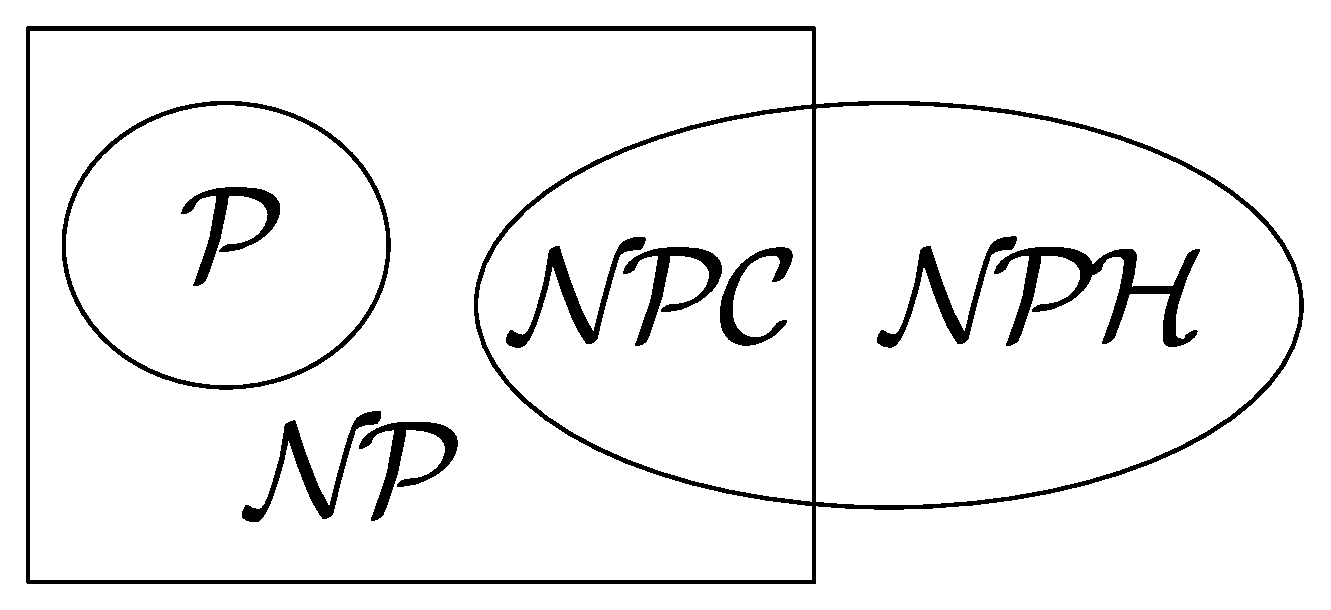
\includegraphics[width=0.5\textwidth]{images/title/P-NP-NPC-NPH问题关系图.pdf}
		\caption{P-NP-NPC-NPH问题关系图}
		\label{fig:P-NP-NPC-NPH问题关系图}
	\end{figure}
\end{homeworkProblem}



\begin{homeworkProblem}
	对于给定$x\neq 0$, 求$n$次多项式$P(x)=a_0+a_1x+a_2x^2+\cdots+a_nx^n$的值.
	\begin{itemize}
		\item 设计一个最坏情况下时间复杂度为$\Theta(n)$的求值算法;
		\item 证明任何求值算法的时间复杂度都是$\Omega(n)$.
	\end{itemize}
	\solution \,\,(1). 采用秦九韶算法, 递归计算如下:
	\begin{align}
		P_0\left( x \right) &=a_n \notag
		\\
		P_1\left( x \right) &=P_0\left( x \right) \cdot x+a_{n-1} \notag
		\\
		P_2\left( x \right) &=P_1\left( x \right) \cdot x+a_{n-2} \notag
		\\
		P_3\left( x \right) &=P_2\left( x \right) \cdot x+a_{n-3} \notag
		\\
		&\vdots  \notag
		\\
		P_n\left( x \right) &=P_{n-1}\left( x \right) \cdot x+a_{n-3} \notag
	\end{align}
	上述算法用一个for循环就可以实现, 并且循环体內部的操作就只有加法和乘法, 即循环体消耗常数时间并且循环次数为$n+1$. 因此算法在最坏情形下的时间复杂度为$\Theta(n)$.

	(2). 多项式$P(x)$有$n+1$个系数, 对于任意一个算法$\mathcal{A}$, 都需要对\textbf{每一个系数}至少做一次处理, 否则算法就可能得到错误的输出. 即任何正确的算法都至少需要$n+1$次运算, 即最坏情况下的时间复杂度下界为$\Omega(n)$.
\end{homeworkProblem}

\begin{homeworkProblem}
	写出下述优化问题对应的判定问题, 并证明这些判定问题$\in \mathcal{NP}$:
	\begin{itemize}
		\item \textbf{最长回路优化问题}: 任给无向图$G$, 在$G$中找到一条最长的初级(即顶点不重复的)回路.
		\item \textbf{图着色优化问题}: 任给无向图$G=(V,E)$, 给$G$的每一个顶点涂一种颜色, 要求任一条边的两个端点的颜色都不相同. 如何用最少的颜色给$G$的顶点着色? 即求映射$f:V\to \mathbb{Z}^{+}$满足条件$\forall (u,v)\in E,f(u)\neq f(v)$, 且使$\text{card}\left\{ f\left( u \right) |u\in V \right\}$最小.
	\end{itemize}
	\solution 上述优化问题对应的判定问题为:
	\begin{itemize}
		\item \textbf{最长回路判定问题}: 任给无向图$G=(V,E)$和正整数$L\leq |V|$, 在$G$中能否找到一条长度$\geq L$的初级(即顶点不重复的)回路?
		\item \textbf{最长回路判定问题}的非确定性多项式时间算法$\mathcal{A}$: 猜想对$G$的任意一条初级回路$C$, 若$C$的长度$\geq L$, 则回答“yes”, 否则回答“no”. 显然该问题$\in \mathcal{NP}$.
		\item \textbf{图着色判定问题}: 任给无向图$G=(V,E)$和正整数$K$, 给$G$的每一个顶点涂一种颜色, 要求任一条边的两个端点的颜色都不相同. 能否用不超过$K$种颜色给$G$的顶点着色? 即是否存在映射$f:V\to \mathbb{Z}^{+}$满足条件$\forall (u,v)\in E,f(u)\neq f(v)$, 且使$\text{card}\left\{ f\left( u \right) |u\in V \right\}\leq K$?
		\item \textbf{图着色判定问题}的非确定性多项式时间算法$\mathcal{B}$: 猜想用不超过$K$种颜色给$G$的每一个顶点涂色, 检查每一条边的两个端点的颜色是否都不相同. 若是, 则回答“yes”, 否则回答“no”. 即猜想一个单射$f:V\to \left\{ 1,2,\cdots,K \right\}$, 若满足条件$\forall (u,v)\in E,f(u)\neq f(v)$, 则回答“yes”, 否则回答“no”. 于是可知该问题$\in \mathcal{NP}$.
	\end{itemize}
\end{homeworkProblem}

% 引用文献
\bibliographystyle{unsrt}  % unsrt:根据引用顺序编号
\bibliography{refs}


\end{document}
